\section{Cardiac Anatomy and Physiology}
\label{sec:intro_physiology}
In this section we will give a very short introduction to cardiac
physiology, and explain some of the basic terms used in this
thesis. The reader is referred to the book of Arnold M. Katz for 
more details \cite{katz2010physiology}.


\subsection{Myocardial structure and morphology}
The heart is the muscular organ responsible for circulating blood
throughout the body. Figure \ref{fig:heart_anatomy} shows a schematic
representation of the heart. 


\begin{figure}[htbp]
  \centering
    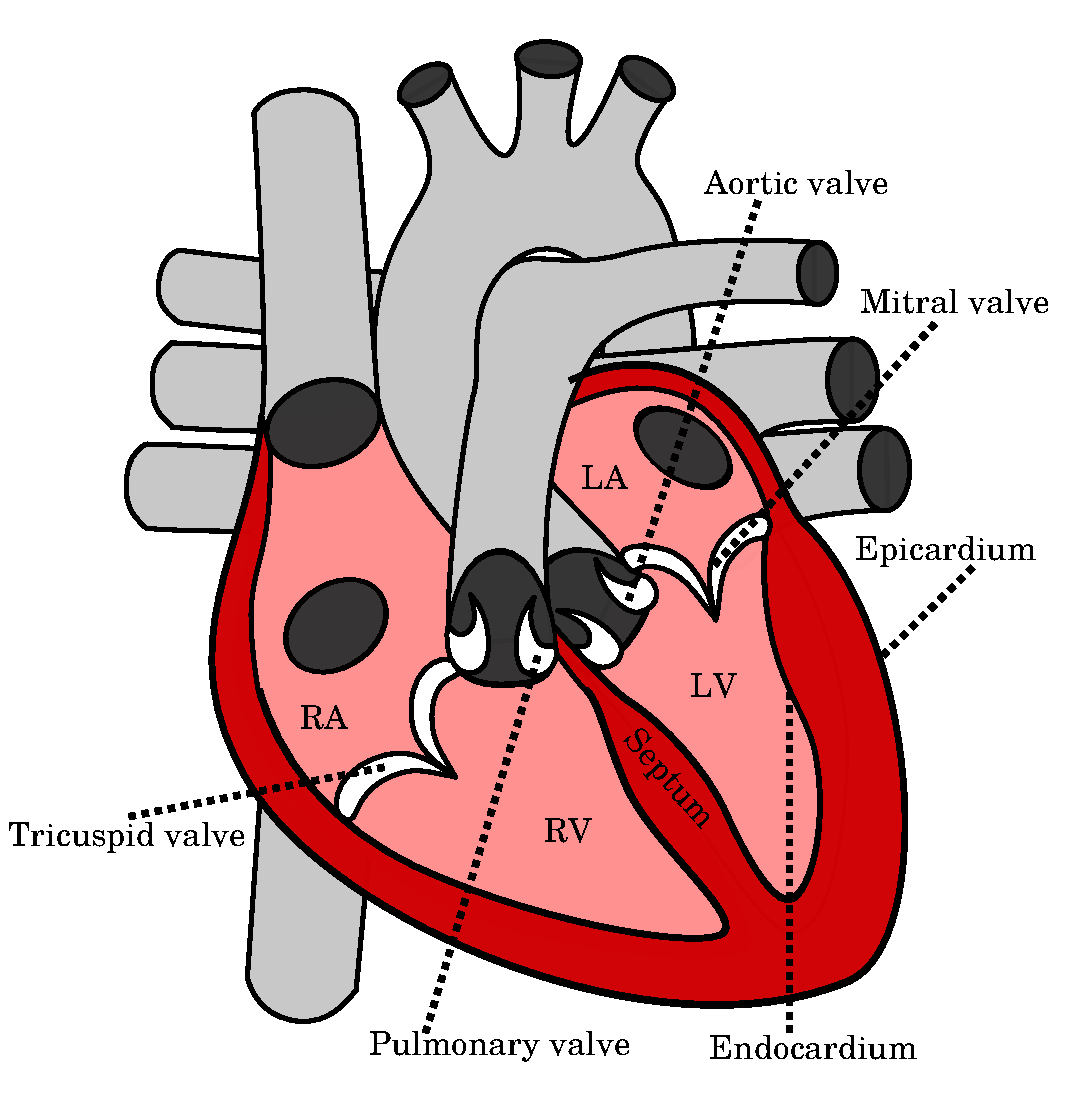
\includegraphics[width=0.7\textwidth]{chapters/introduction/figures/heart_anatomy.pdf}
\caption{Schematic representation of the heart's anatomy. (Adapted and modified from Wapcaplet in Sodipodi).}
\label{fig:heart_anatomy}
\end{figure}


Deoxgenated blood is transported from the body trough the veins and to
the right atrium (RA). From the RA, blood flows to the right ventricle
(RV), before it is sent through the the pulmonary arteries(PA) and to the
lungs, where the bloods gets oxygenated. From the lungs, the blood
travels through the pulmonary veins to the left atrium (LA), and
finally to the left ventricle (LV), before is is sent out to the body
again through the aorta.

The flow from one chamber to another is driven
by pressure gradients, that is blood flows from regions with higher
pressure to regions with lower pressure. Consequently, the lowest
pressure is found in the veins entering the heart, and the highest
pressure is found in the left ventricle. Between the different
chambers there are valves that open and close in response to pressure
gradients as illustrated in Figure \ref{fig:heart_anatomy}.


The heart itself is located approximately in the center of the chest
with the \emph{apex} of heart angled down towards the left of the
body, and the \emph{base} located just behind the breastbone.


Starting from the outside of the heart we have the \emph{pericardium},
the \emph{epicardium}, the \emph{myocardium} and the \emph{endocardium}. 
The endo- and epicardium are respectively the inner and outer layers of the
myocardium. The myocardium is made up by individual muscle cells, or
myocytes, which branch and join neighboring cells, and form a
complicated fibrous network which is often referred to as a 
\emph{functional syncytium} (meaning that the number of active muscle
fibers cannot be varied from beat to beat). Each myocyte is composed
of bundles of myofibriles, which again contains
\emph{myofilaments}. The myofilaments consist of a repeated pattern
of lines and bands which can be seen as a collection of individual
contractile units called \emph{sarcomeres}. A simple sketch of a
sarcomere is shown in Figure \ref{fig:sarcomere}. 
\begin{figure}[htbp]
  \centering
    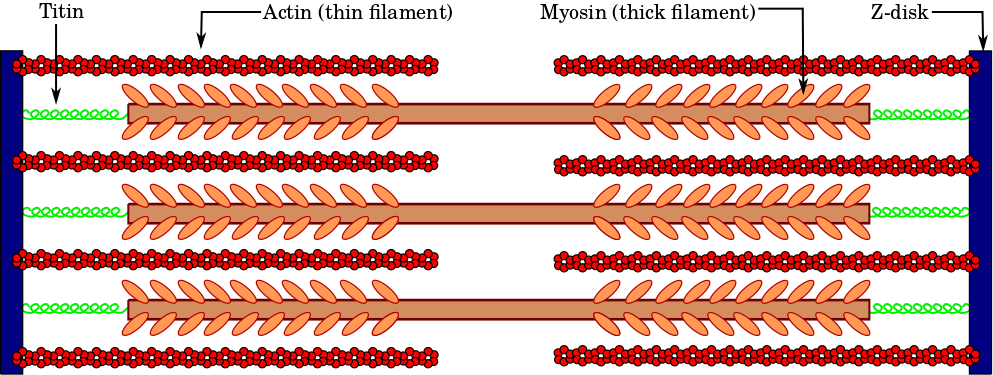
\includegraphics[width=1.0\textwidth]{chapters/introduction/figures/Sarcomere.png}
\caption{Illustration of the sarcomere structure.}
\label{fig:sarcomere}
\end{figure}

The sarcomeres are composed thick and thin filaments that slides
back and forth when the muscle contracts or relaxes.
The thin filaments are made up by a protein called \emph{actin} while
the thick filaments are made up by a protein called \emph{myosin}.

\subsection{The cardiac cycle}
\label{sec:cardiac_cycle}

The heart beats in a cyclic manner, about one beat every second.
The contraction of the heart is triggered by an electrical signal called an action
potential originating from specialized cells in the right atrium. When an action
potential is triggered, calcium is released into the cells. These
calcium ions binds to a complex called troponin C located at the thin
filaments, which then exposes the actin to the myosin head. When
myosin binds to actin we say that a \emph{cross-bridge} is formed
between the thin and thick filaments. A \emph{power stroke} is
triggered after ATP hydrolysis, and the sarcomere shortens. 
The signal propagates through the myocardium and along
specialized electrical highways with high conducting cells.

% One way to describe the cardiac cycle is via the \emph{electrocardiogram}
% (ECG), which is a way of measuring the electrical propagation though
% the heart. Another
One way to describe the cardiac cycle is by means of
the pressure and volume inside the chambers. For example, plotting
the left ventricular (LV) volume on the $x-$axis and the LV pressure on the $y-$axis
provides an intuitive representation of the cardiac cycle known as the
\emph{PV-loop}. In Figure \ref{fig:pv_loop} we show an illustration of
a typical PV-loop. At end-diastole (ED), the mitral valve closes, and
the ventricle contracts against a rising pressure. During this phase,
no blood goes in or out of the ventricle and we call it the
\emph{isovolumic contraction} phase. When the
ventricular pressure exceeds the aortic pressure, the aortic valve
opens and the heart \emph{ejects} blood into the body. When the ventricular
pressure drops below the aortic pressure, the aortic valve closes and
pressure is dropping as the ventricle is relaxing, and we enter the
\emph{isovolumic relaxation} phase. The phase when the ventricle
contracts, from end diastole until the end of ejection is called
\emph{systole}, hence this point in the cycle is also know as
end-systole (ES). Similarly, the phase for which the ventricle
relaxes from the beginning isovolumic relaxation to end diastole, is
called \emph{diastole}. When the pressure drops below the atrial pressure 
the mitral valve opens and blood is sucked into the ventricle. In the
final stage of the filling of the ventricle, the atria contracts and
fills the ventricle before we arrive at end-diastole, and the cycle
repeats. The phase of atrial contraction is also known as atrial
systole. 


\begin{figure}[htbp]
  \centering
    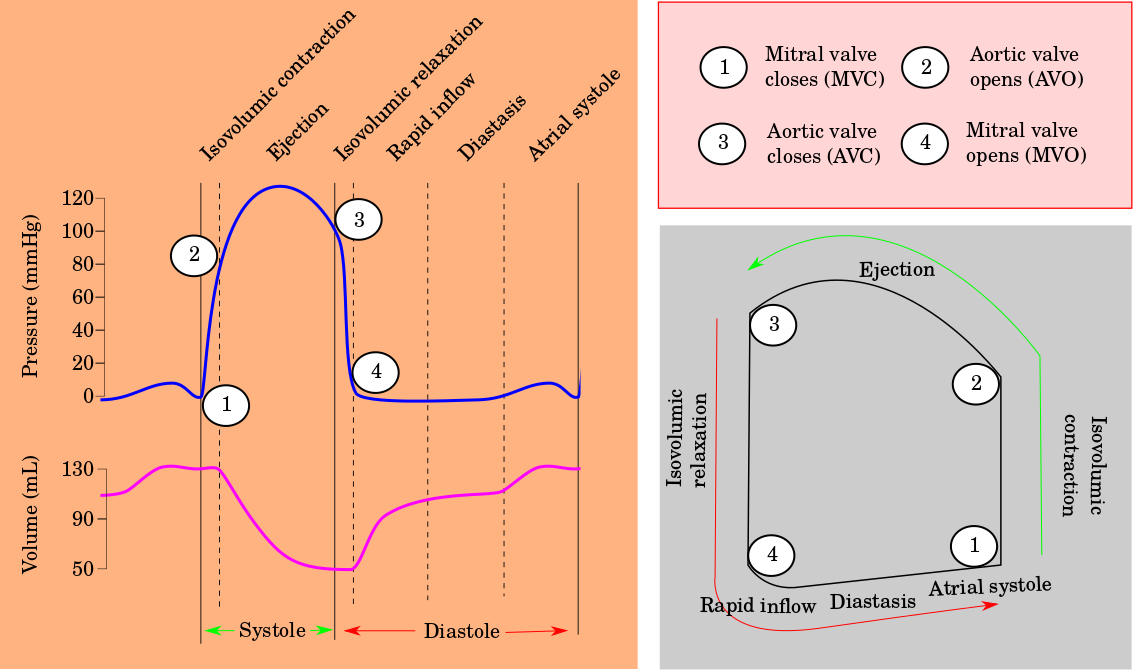
\includegraphics[width=0.85\textwidth]{chapters/introduction/figures/cardiac_cycle.png}
\caption{Showing the relation between pressure and volume in the left
  ventricle during the cardiac cycle. To the left we show the a reduced version of
the classical Wiggers diagram with pressure and volume plotted against
time. To the right we show the pressure volume loop
with volume plotted on the $x-$axis and pressure on the $y-$axis. }
\label{fig:pv_loop}
\end{figure}


% A couple of terminologies used throughout 
\subsection{Ventricular pumping function}
\label{sec:ventricular_pumping_function}



The pressure and volume inside the ventricle can provide us with
information about the passive and active properties of the
myocardium. Imaging it was possible to shut down all contractile
units in the myocardium, and remove all loads (e.g set the pressure
to zero). This would be analogous to have a deflated balloon. In order to
get some information about the stiffness of the myocardium one could
try to inflate the ventricle. The stiffer the myocardium is, the
higher pressure would be needed in order to increase the volume.
This relationship between the pressure and volume during the inactive
state is called the end diastolic pressure volume relationship
(\emph{EDPVR}).

Similarly, imaging now that the ventricle is at the end-systolic state,
when the muscle cells are contracting at its most forcefully. Changing
the pressure at this state would also result in a change in volume and
this relationship between pressure and volume  is called the end
systolic pressure volume relationship (\emph{ESPVR}). The two pressure
volume relationships are depicted in Figure \ref{fig:intro_pvr}.

\begin{figure}[htbp]
  \centering
    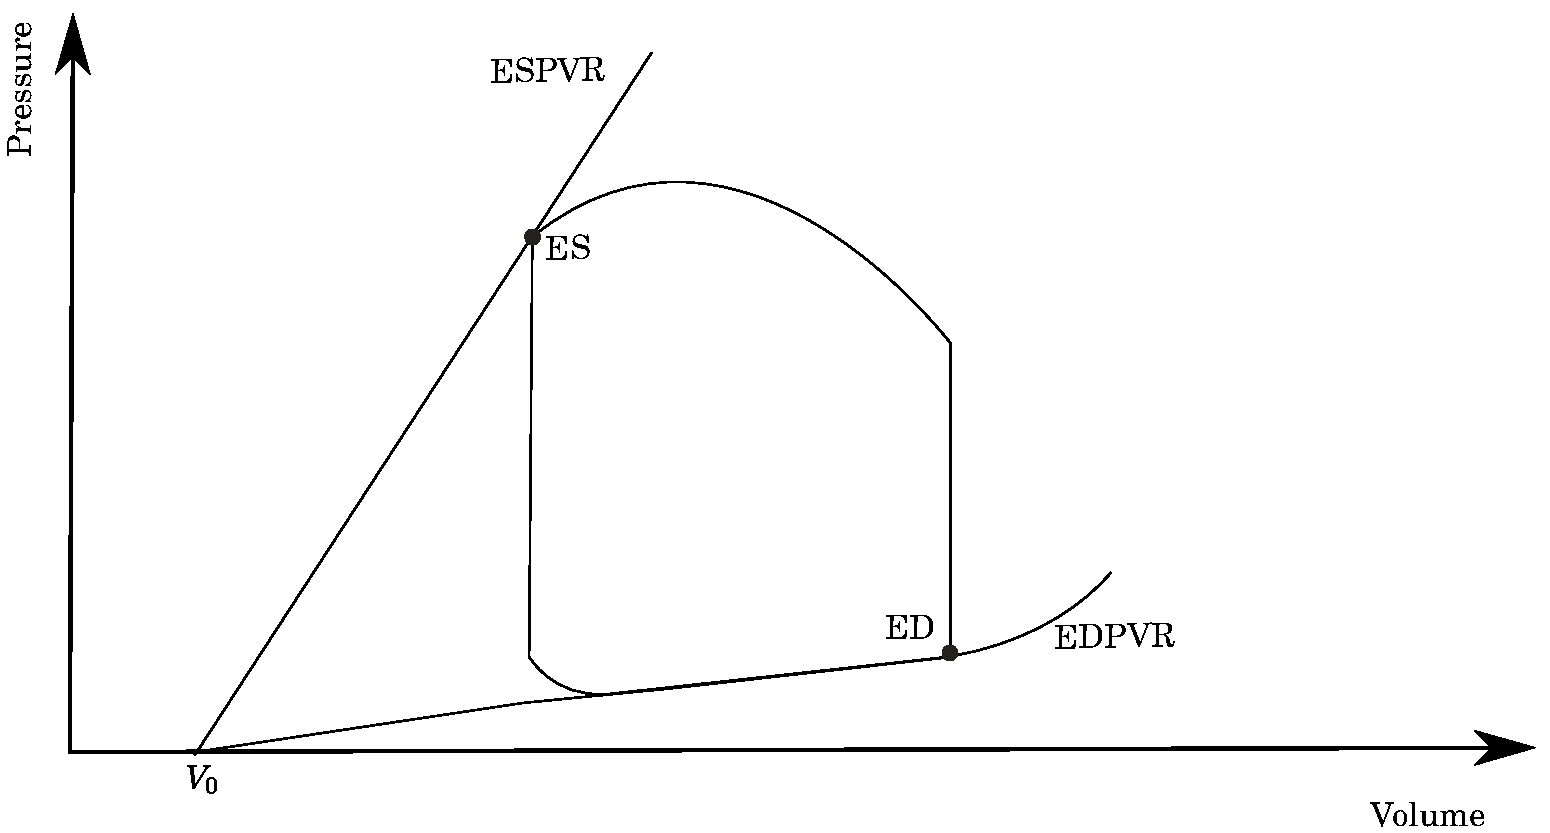
\includegraphics[width=\textwidth]{chapters/introduction/figures/pvr.pdf}
\caption{Illustration of the end diastolic pressure volume
  relationship (EDPVR) and the end systolic pressure volume
  relationship (ESPVR). The volume axis intercept $V_0$ from the time
  varying elastance model is also shown. }
\label{fig:intro_pvr}
\end{figure}




Although single-beat estimation of these relationships do
exist \cite{senzaki1996single,klotz2006single}, the EDPVR and ESPVR
can be estimated by changing the loading condition.
Changing the \emph{preload}, i.e the load on the ventricle
before it starts contracting would brings us along the EDPVR
curve, while changing the \emph{afterload}, i.e the load after
the ventricle has contracted, would shift the end-systolic point along
the ESPVR curve.


The ventricular pumping function depends on the loads that the
ventricle experience. If the amount of blood returning from the veins
into the heart increases, i.e increased preload, the end diastolic
volume increases and the ventricle contracts more forcefully in order
to synchronize the amount of ejected blood with the venous
return. This fundamental law, is called the \emph{Frank-Starling
  law}. The Frank-Starling law relates the EDPVR to the ESPVR, and
states that the stroke volume, i.e the difference in end systolic and
end diastolic volume, increases in response to and increase in
preload. This allows the cardiac output to
be synchronized with the venous return and blood supply, without
depending upon external regulation. 


The slope of any pressure volume relationship is called the \emph{elastance},
and a famous model known as the  time varying elastance model, relates
a time varying elastance $E(t)$ to the pressure and volume in the ventricle
\cite{sagawa1977end},  
\begin{align}
  P(t) = E(t)( V(t) - V_0 ).
  \label{eq:time_varying_elastance}
\end{align}
Here $P$ is the endocardial pressure, $V$ the cavity volume, $E$ the
time-varying elastance, and $V_0$ the volume axis intercept.

In fact, the end systolic elastance, $E(t)$ with $t$ being time of end
systole, is considered to be the gold
standard in terms of quantifying myocardial \emph{contractility}.
However, it is rarely used because it is difficult to determine
clinically. What should be noted is that end systolic elastance is
independent of load, and therefore serve as measure of the ability of
the ventricle to do work, i.e myocardial contractility.







% 



% % The Starling Curve is a plot of the ESPVR - EDPVR, showing that the
% % output increases up to some maximum (at the ascending limb). Thereafter
% % it decreases on the descending limb. If the sarcomeres works on the
% % descending limb, the heart would dilate and become weakened.


% Stroke volume, cardiac output. 







% \subsection{Myocardial Contractility}

% Contractility can be seen as the manifestation of all the factors that
% influence the interactions between the contractile proteins.
% One simple definitions is \emph{myocardial contractility is the
%   ability of the heart to do work}. A change in myocardial
% contractility can be seen if there is a change in ejection which is
% not caused by changes in the initial fiber length (ED). If the end
% diastolic volume remains the same, but the stroke work changes there
% is a change in contractility.

% Under normal circumstances, the myocardial cells generate less than
% half the of their maximal contractility. One could increase the
% contractility by providing more calcium to the cells.


% In order to find a suitable index for myocardial contractility we take
% step back and consider Hills postulate: \emph{the ``active points'' of
%   muscle can exist in two states: 1. active points are maintaining
%   tension, 2. the active points are participating in a chemical
%   reaction.} 
% If the muscle is presented with a heavy load, developed tension is
% high, shortening velocity is low and the load is only moved a short
% distance. In this case the active points are holding tension.
% On the other hand, if the muscle is presented with a light load, the
% shortening velocity is high and the load is moved a longer
% distance. In this case more of the active points are participating in
% chemical reactions. 
% In both cases, the contractility might be the same which is why we
% need a load independent measure of contractility.
% Looking at the force-velocity relationship we can say that the maximum
% force (tension) is achieved when all the active points are holding
% tension ($P_0$). $P_0$ is proportional to the number of active
% cross bridges.
% Similarly, the maximum velocity is achieved when all
% the active points are participating in a chemical reaction
% ($V_{\text{max}}$). $V_{\text{max}}$ reflects the maximal rate of
% cross bridge cycling. 
% This is explained by the Hill equation, which
% relates the force to velocity, and the intercepts are $P = P_0, (V = 0)$
% and $V = V_{\text{max}}, (P = 0)$. This is very difficult to meause in
% cardiac cells because cariac muscle cells are not tentanized.

% The most commonly used index of contractility was formalized
% \cite{sagawa1977end} using a time varying elastance model, which
% states that at any point in the cardiac cycle the pressure and volume
% are linearly related by the time-varying elastance, or formally:
% \begin{align}
%   P(t) = E(t)( V(t) - V_0 ).
%   \label{eq:time_varying_elastance}
% \end{align}



\subsection{Cardiac Pathophysiology}
Pathophysiology is the study of the physiology of the diseased heart,
and we will briefly mention some of the different cardiac diseases
encountered in this thesis. 


\subsubsection{Heart failure}
Heart failure is a common term for all heart diseases in which the
heart in unable to supply the body with enough blood to meet its demand.
% Consequently, patients suffering from heart failure has a reduced
% cardiac output. It is common to distinguish between systolic and
% diastolic heart failure. 

\subsubsection{Left bundle branch block}

One type of heart failure can result from conduction block in the
heart. The action potential travels through these electrical highways
of high conducting cells. One of these highways known as the Bundle of
His splits into two parts, the right and left bundle. The right bundle
activates the right ventricle, while the left bundle activates the
left ventricle. For patients suffering from left bundle branch block,
there is ``road block'' on the highway along the left bundle, meaning
that the left ventricle is activated later than preferable, and the
right ventricle is activated prior to the left
ventricle. This can result in a dyssynchronous contraction, yielding a
reduced pumping effect. A promising treatment for this patients is
called Cardiac Resynchronization Therapy (CRT) \cite{cleland2005effect}.

Imagine a boat with rowers on both sides trying to get the boat moving
forward. If the rowers don’t synchronize their strokes, the boat will
veer from side to side and have a much longer route – if it gets
anywhere at all. To synchronize the rowers, we could add a coxswain
who tells the rowers when to row. We can use the rower analogy to
think of the contractions of the left and right side of the
heart. With the heart, implanting a CRT device is like adding a
coxswain to direct the rowers. The CRT’s goal is to try to
resynchronize the heart so that the left and right ventricles contract
simultaneously. It involves pacing the heart on both the left and
right ventricle so that the heart can contract in a synchronous
way. Therefore CRT are often referred to as biventricular pacing, or
just BiV pacing.

Experiments show that between 30-40\% of the selected patients do
not respond to CRT \cite{daubert20122012}, which is why much research
is put into increasing the responder rate. 



\subsubsection{Pulmonary hypertension}


\subsection{Summary of Cardiac Physiology}
The multiscale and multiphysics phenomena governing the mechanics of
the heart is complex. How the molecular dynamics should be coupled to
the electrophysiology at the cellular level, how the electrophysiology
should be coupled to the mechanics at the organ level and what type of
feedback mechanisms that should be included is far from fully
understood. In this thesis we limit ourselves to the study of what is
happening on the organ level, and concentrates purely on the
mechanics. 


%%% Local Variables:
%%% mode: latex
%%% TeX-master: "../../main"
%%% End:
